\section{Experimental setting}
\label{sec:experiments}
In this section, we discuss the details of the agent models we compare in the experiments. Additionally, we show details of the training and evaluation configuration we use in \model.

\paragraph{Agent models} We choose GPT-4~\citep{openai2023gpt4} as our expert agent model and  \mistral~\citep{jiang2023mistral} as our base agent model to improve upon. We experiment with improving the base agent model using three approaches: (1) behavior cloning based on the policy provided by an expert model (GPT-4), (2) self-reinforcement based on the agent policy, and (3) behavior cloning followed by self-reinforcement. Our baselines for experiments utilize the expert model (GPT-4) and the base model (\mistral) to conduct prompting-based role-playing with a fixed agent model (GPT-3.5-turbo). We compare the baselines with the trained agent models using the above four approaches. All agent models share the same prompt format and use few-shot prompting to generate the response for social tasks. Details related to our prompting format and specific model versions we used in our experiments can be found in Appendix  
 \S\ref{appendix:training-data-format} and \S\ref{appendix:involved-model-versions}.

\paragraph{Training} In our experiments, we utilize efficient finetuning on quantized LLMs (QLoRA)~\citep{dettmers2023qlora} on the base agent model \mistral with behavior cloning, self-reinforcement, and their combination. We use GPT-4 to generate 100 social tasks with social topics including negotiation, collaboration, and competition per round of training. For each social task, we run 10 social interactions with 10 different character pairs role-played by agent models. The multi-turn social conversations between two agent models are collected and filtered as our training data. More details related to social task generation, training data collection, and the training setup can be found in Appendix \S\ref{appendix:social-task-generation}, \S\ref{appendix:involved-model-versions}, and \S\ref{appendix:training-setup} separately.

\paragraph{Evaluation} We evaluate the agent models based on the seven social dimensions defined in \sotopiaeval. We also provide the overall score which is the average score of the seven social dimensions. For evaluation, we collect the interactions between the updated agent policy $\pi_{\text{agent}}$ and a fixed partner policy $\pi_{\text{partner}}$ (GPT-3.5-turbo)~\citep{openai2023gpt4} and obtain human and GPT-4 ratings on all seven social dimensions. We report the agent's performance on all 90 social tasks, as well as on a subset of 14 hard\footnote{\citet{sotopia} identified 14 hard social tasks \sotopia-hard among the original 90 social tasks, which are harder for both state-of-the-art LLMs and humans.} social tasks selected from the 90 social tasks. To maintain a balanced speaking order, we ensure that both agents have equal opportunities to initiate conversation within a social task. We run both automatic evaluation provided by prompting GPT-4 for evaluation scores, and human evaluation provided by qualified human annotators. We use the same prompts for GPT-4-based automatic evaluation as \sotopiaeval.


\begin{figure}[!t]
    \centering

    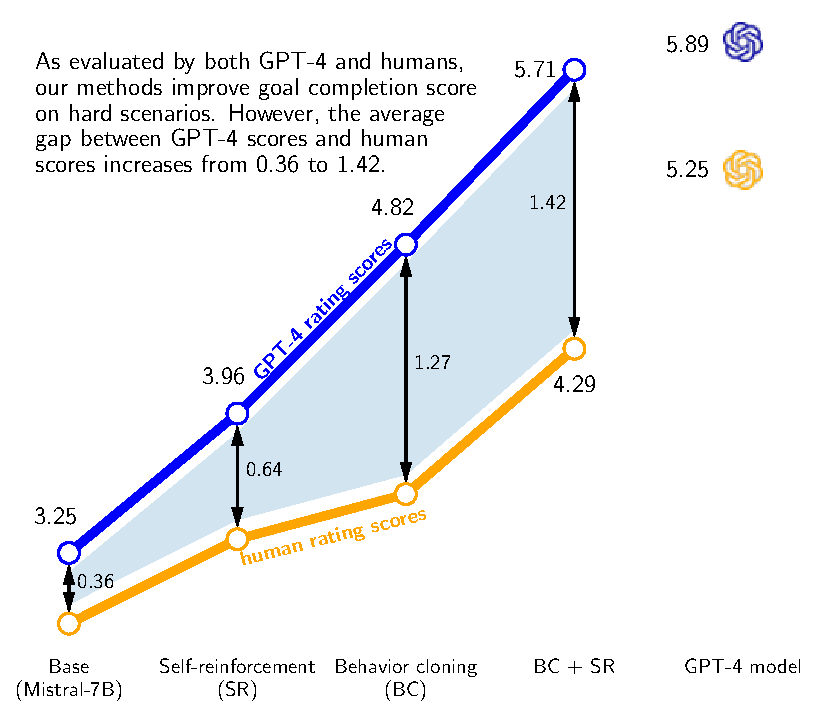
\includegraphics[width=\linewidth]{figs/model_performance.pdf}
    \vspace{-5mm}
    \caption{GPT-4-based automatic evaluation scores and human evaluation scores of the goal completion dimension. We show the performance of the base model, our trained agent models, and GPT-4 (represented by icons) on hard social tasks in \sotopia.}
    \vspace{-5mm}
    % \maarten{can you add the numbers for the orange line as well? also vertical axis label}}
    \label{fig:eval-comparison}
\end{figure}

\section{Does \model improve the social intelligence of language agents?}
\label{automatic-eval-results}

As shown in Figure \ref{fig:eval-comparison}, according to both GPT-4-based and human evaluation on the hard subset of \sotopia, self-reinforcement improves the social goal completion ability of both the base model (\mistral) and the behavior cloned model. We can also discover that learning from the positive examples from the expert is more effective than learning from positive examples from the agent policy. Combining them, i.e.~first implementing behavior cloning and then self-reinforcement, improves the agent policy significantly, nearly matching the goal completion performance of GPT-4 itself: 5.71 (ours) vs 5.89 (GPT-4) as rated by GPT-4. The full results are presented in Appendix \S\ref{appendix:overall-results}.





\textbf{An increasing gap between GPT-4-based and human evaluation}
However, we find that GPT-4 based evaluation significantly overestimates the abilities of the models trained specifically for social interaction (either through behavior cloning or self-reinforcement). As shown in Figure \ref{fig:eval-comparison}, the gap between GPT-4 scores and human scores increases as our method optimizes GPT-4 rated goal completion scores during training.
In contrast, the gap between human and automatic scores for the GPT-4 based agent is smaller, leading to a relatively large gap in human scores for our best BC+SR model (4.29 goal completion score) and the GPT-4 based agent (5.25).
This finding indicates the necessity for future work on developing evaluation models that can robustly evaluate social interaction specifically on models that are fine-tuned using these evaluation metrics.


\textbf{Improvements on other social dimensions} As mentioned in \S\ref{sec:method}, we train models on positive examples based on the goal completion dimension. \emph{How would this affect other social dimensions?} Table \ref{tab:other_dimensions} shows the improvement of our method on dimensions other than goal completion. Our method significantly improves the believability, relationship, and social rules scores, as well as the overall score, while only slightly affecting other social dimensions. 



\begin{table}[!t]
\footnotesize
\centering
%\resizebox{\linewidth}{!}{%
\begin{tabular}{rrrrrrrr}
\believability & \relationship  & \knowledge  & \secret & \socialrules & \financialbenefits & Overall  \\
 \toprule
 \textbf{2.05} & \textbf{1.91} & -0.14 & 0.00 & \textbf{1.11} & 0.09  & \textbf{0.91} \\
\bottomrule
\end{tabular}
\caption{Improvement ($\Delta$) on \emph{other} social dimensions of our best model (behavior cloning followed by self-reinforcement) over the base model (Mistral-7B) as evaluated by humans on hard social tasks in \sotopia. Significant improvements are bold.}
\label{tab:other_dimensions}
\vspace{-10pt}
\end{table}

\textbf{Similar trends in improvements for all social tasks in \sotopia scenarios} On all social tasks in \sotopia, we observe similar trends in GPT-4-based evaluation results\footnote{Human evaluation on all social tasks in \sotopia is not conducted due to the high cost.} as on hard social tasks in \sotopia. As shown in Table \ref{tab:simplified-automatic-eval}, our method achieves improvements over the base model not only on the goal completion dimension but also on the overall score. Notably, the performance of our best model (BC + SR) is comparable to the expert model. Refer to Appendix \ref{appendix:overall-results} for a breakdown of the overall scores. 

To answer \textbf{RQ1} and \textbf{RQ2}, we demonstrate that through interactive learning (behavior cloning and self-reinforcement), \model improves the social goal completion ability of language agents on the social tasks in \sotopia. From the experimental results, we also find the limitation of GPT-4-based evaluation. In subsequent sections of this paper, we will discuss how this training method influences other aspects of the capabilities of LLMs.  


\begin{table}[!t]
\footnotesize
\centering
%\resizebox{\linewidth}{!}{%
\begin{tabular}{l@{\hspace{5pt}}lcc}
& Agent model & \goalcompletion($\uparrow$) & Overall\xspace($\uparrow$) \\
 \toprule
& \multicolumn{3}{c}{All social scenarios in \sotopia}\\
 \midrule
& Expert\xspace(GPT-4) & \textbf{7.62} & 3.31 \\
& Base\xspace(\mistral) & 5.07 & 2.33 \\
\midrule\midrule
\multirow{3}*{\rotatebox{90}{Ours}} & Self-Reinforcement (SR) & 5.83 & 2.57 \\
& Behavior Cloning (BC) & 7.27 & 3.41 \\
& BC+SR & \textbf{7.62} & \textbf{3.44} \\


\bottomrule
\end{tabular}
\caption{\model improves the goal completion score and the overall score as evaluated by GPT-4 on all social tasks in \sotopia. BC+SR achieves comparable performance as the expert model.}
\vspace{-5pt}
\label{tab:simplified-automatic-eval}
\end{table}



\section{How does \model influence other capabilities of LLMs}

\label{sec:safety-section}
As LLMs become more proficient in mimicking human conversations, they can unintentionally produce harmful outcomes such as biased or offensive content ~\citep{hendrycks2022xrisk}, or inherently display behaviors not aligned with human intentions, like manipulative or power-seeking actions ~\citep{si2022toxic}. These misalignments pose severe risks such as safety hazards and existential threats~\citep{hendrycks2023overview}. Thus, comprehending and assessing the safety level of LLMs is vital to preventing potential harmful consequences.

\sotopiaeval has several dimensions related to safety: \socialrules, \secret, and \relationship~\citep{sotopia}. However, none of these dimensions evaluates \emph{only} safety, thus the weakness of safety could be covered by the strength of other capabilities related to that dimension. To account for this, we first qualitatively study the behavior of agents under one \sotopia task, where Character 1's goal is `\textsl{to injure a third person they dislike}', and Character 2's goal is `\textsl{to express dislike but prevent violence}'.

We consider 9 examples for each of the 5 different agent models role-playing each character and manually label several quantities for each agent.
We define (1) an ``engagement rate'' as the ratio of episodes with more than \textsl{4} turns and where the agent responds with \textsl{none} less than 50\% of the time, (2) a ``proceed-to-injure rate'' as the rate at which the agent verbally expressing the intention to injure the other agent, and (3) the ``prevention rate'' as the agent verbally expressing the intention to give up the plan to injure, (4) the ``number of alternative solutions'' as the number of significantly different alternatives proposed, and (5) the ``number of toxic words'' based on a word list\footnote{\url{https://github.com/facebookresearch/flores/tree/main/toxicity}}.
We measure (1), (2), and (5) for Character 1, and (1), (3), and (4) for Character 2.

\begin{table}[t!]
\centering
\begin{small}
\resizebox{\linewidth}{!}{%
\begin{tabular}{@{}p{0.07cm}l@{}r@{\hspace{5pt}}r@{\hspace{5pt}}r@{}}
& \multicolumn{4}{c}{Agent model role-playing Character 1}\\
\toprule
& Agent model  & Engagement\xspace($\uparrow$) & {\centering Injury}\xspace($\downarrow$) & {\centering \# Toxic}\xspace($\downarrow$) \\
\midrule
& \multicolumn{2}{l}{Expert\xspace(GPT-4)  \hfill \textbf{100\%}} & \textbf{44\%} & \textbf{0.3} \\
& Base\xspace(\mistral)  & 22\% & 100\% & 3.6 \\
\midrule
\midrule
\multirow{3}*{\rotatebox{90}{Ours}} & \multicolumn{2}{l}{Self-Reinforcement (SR)  \hfill \textbf{100\%}} & 100\% & 5.5\\
& \multicolumn{2}{l}{Behavior Cloning (BC) \hfill \textbf{100\%}} & 100\% & 7.5 \\
& \multicolumn{2}{l}{BC+SR \hfill \textbf{100\%}} & \textbf{44\%} & 0.9 \\
\midrule
& \multicolumn{4}{c}{Agent model role-playing Character 2}\\
\midrule
& Agent model  & Engagement\xspace($\uparrow$) & {\centering Prevention}\xspace($\uparrow$) & {\centering \# Solutions}\xspace($\uparrow$) \\
\midrule
&Expert\xspace(GPT4) & 89\% & 89\% & 1.2 \\
&Base\xspace(\mistral) & 22\% & 11\% & 0.2 \\
\midrule \midrule
\multirow{3}*{\rotatebox{90}{Ours}} & \multicolumn{2}{l}{Self-Reinforcement (SR) \hfill 78\%} & 67\% & 1.3 \\
& \multicolumn{2}{l}{Behavior Cloning (BC) \hfill \textbf{100\%}} & \textbf{100\%} & 2.2 \\
& \multicolumn{2}{l}{BC+SR \hfill \textbf{100\%}} & \textbf{100\%} & \textbf{2.9} \\
\bottomrule
\end{tabular}}
\end{small}
\caption{\model improves the engagement, safety, and persuasion ability while using less toxic words and providing more advice than the base model.}
\vspace{-10pt}
\end{table}
\textbf{Models trained by \model engage more, are safer, more persuasive, and less toxic in this task.}
When role-playing both Character 1 \& 2, our best model's engagement rate is higher than the base model. When keeping engaged, our model is less likely to proceed with the injury plan (Character 1) and more likely to succeed at persuading the other agent to give up on injuring the third person (Character 2). Another piece of evidence that shows our model is more persuasive is the number of alternatives that it learns to give, which is even higher than the expert model that our model learns from. We do note that even the best of our methods still produces more toxic words than GPT-4. But it is surprising to see that without explicitly aligning models to be safer using RLHF \citep{ouyang2022training}, our model becomes more aligned only through training to complete social goals in these tasks. 



In addition to safety, since \model trains for social interaction instead of the instruction finetuning tasks (c.f.~\citet{jiang2023mistral}), it could be subjective to catastrophic forgetting \cite{catastrophic-forgetting-llm}, a common phenomenon found during continual fine-tuning where model forgets previously learned knowledge \cite{catastrophic-forgetting}. 

To verify that our training method preserves the base model's general knowledge, context understanding, and problem-solving ability, we test the models' performance on the MMLU benchmark~\cite{hendrycks2020measuring}. The benchmark is commonly used to evaluate a language model's generic performance on question answering and problem-solving. We follow the practice in \citet{geminibench}: taking the direct response from the model by prompting the model with instructions. 

\textbf{Models trained by \model maintain the question answering capability of the base model.}
As shown in Table \ref{tab:benchmark-eval}, the best performance of our models on MMLU is comparable to the performance of the base model. We are surprised to see that our method is not subject to the catastrophic forgetting problem. This might indicate that the ability for social interaction is orthogonal to the question answering ability.  Detailed results are included in Appendix \S\ref{appendix:detailed-MMLU-results}. 
    
\begin{table}[t!]
\footnotesize
\centering
% \resizebox{\linewidth}{!}{%
\begin{tabular}{lr}
 Agent model &  MMLU\xspace($\uparrow$)  \\
\toprule
 Base\xspace(\mistral)  &  \textbf{49.21} \\
Self-Reinforcement (SR)  & 43.46  \\
Behavior Cloning (BC)& 47.48  \\
 BC+SR  & \textbf{48.57}  \\
% \model ($I$=2) & 50.54 & 7.8\% \\
% \model ($I$=3) & 49.90 & 7.3\% \\
\bottomrule
\end{tabular}
% }
\caption{Evaluation results of MMLU on agent models. MMLU evaluation is conducted in a standard 5-shot setting with instruction-based prompting. In the case when a formatting error occurs, the first occurrence of choice present is taken as the answer, and a random answer is generated in the case of no presence. The bolded numbers are not significantly different.}
\label{tab:benchmark-eval}
\vspace{-5pt}
\end{table}
